\documentclass[fontset=windows]{article}
\usepackage[margin=1in]{geometry}
\usepackage{ctex}
\usepackage{setspace}
\usepackage{lipsum}
\usepackage{graphicx}
\usepackage{caption}
\usepackage{subcaption}
\usepackage[colorlinks=true,linkcolor=red]{hyperref}

\graphicspath{{figures/}}

\title{\heiti\zihao{2} MOS Characteristics \uppercase\expandafter{\romannumeral2}}
\author{\songti zrrraa}
\date{2023.11.14}

\begin{document}
\maketitle
\thispagestyle{empty}

\section*{I/V Characteristics}

\subsection*{Case \uppercase\expandafter{\romannumeral1}: $V_{DS}<V_{GS}-V_{TH}$}
Last day we know the $I_D-V_{DS}$ relationship when $V_{DS} \leq V_{GS}-V_{TH}$. 

\begin{figure}[htbp]
    \centering
    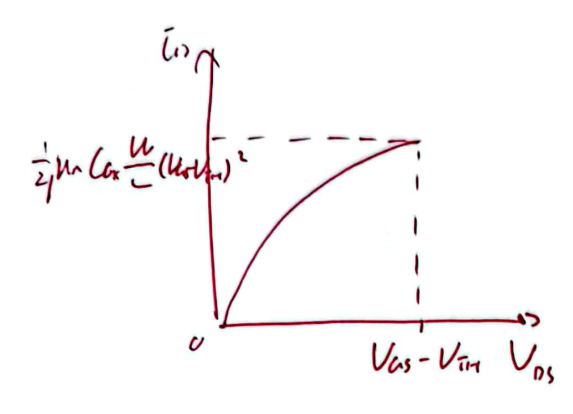
\includegraphics[scale=0.6]{1.jpg}
    \captionsetup{labelformat=empty}
    \caption{The $I_D-V_{DS}$ relationship when $V_{DS} \leq V_{GS}-V_{TH}$}
    \label{1}
\end{figure}

The drain current is: 

$$I_D=\mu_{n}*C_{ox}*\frac{W}{L}[(V_{GS}-V_{TH})*V_{DS}-\frac{1}{2}V_{DS}^2]$$

We now assume that $V_{DS}*(V_{GS}-V_{TH})>>\frac{1}{2}V_{DS}^2$, that is $V_{DS}<<2(V_{GS}-V_{TH})$. 

we can get: 

$$I_D \approx \mu *C_{ox}\frac{W}{L}*(V_{GS}-V_{TH})*V_{DS}$$

That is, $V_{DS}$ is linearly related to $I_{D}$, shows us that 
\textbf{A MOSFET can act as a voltage-dependence resistor}. 
(if $V_{DS}<<2(V_{GS}-V_{TH}$))

\begin{figure}[htbp]
    \centering
    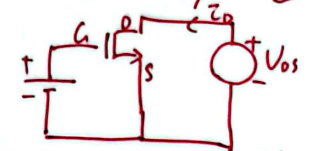
\includegraphics[scale=0.6]{2.jpg}
    \captionsetup{labelformat=empty}
    \caption{$R_{on}=\frac{V_{DS}}{I_D}=\frac{1}{\mu C_{ox}\frac{W}{L}(V_{GS}-V_{TH})}$}
    \label{2}
\end{figure}

$R_{on}$ means the resistance when the MOS turns on. 

\subsection*{MOS Device as a Switch}

\begin{figure}[htbp]
    \centering
    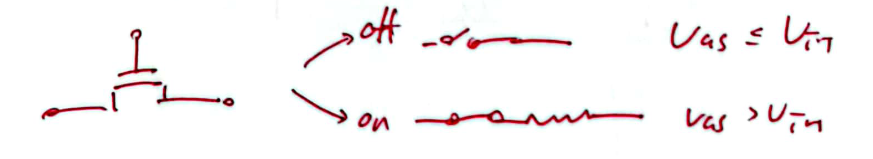
\includegraphics[scale=0.6]{3.jpg}
    \captionsetup{labelformat=empty}
    \caption{MOS device as a switch}
    \label{3}
\end{figure}

For example, it can use in a Bluetooth System, for both side have to determine to transmit or receive.

\subsection*{Case \uppercase\expandafter{\romannumeral2}: $V_{DS}>V_{GS}-V_{TH}$}

\begin{figure}[htbp]
    \centering
    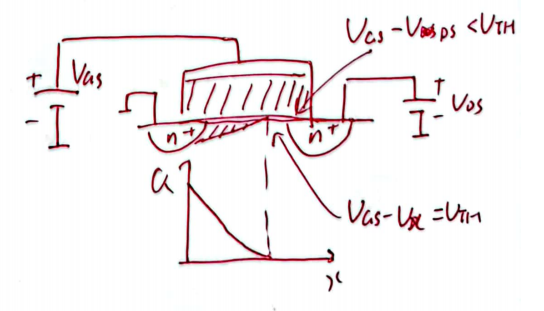
\includegraphics[scale=0.9]{4.jpg}
    \captionsetup{labelformat=empty}
    \caption{Pinch-off}
    \label{4}
\end{figure}

The potential difference between the upper and lower plates at the drain end is less than $V_{TH}$, 
leads to no electronics exit.

We call this phenomenon \textbf{pinch-off}. 

\section*{Rederive I/V Equation}

\subsection*{Relationship between $I_D$ and $V_{DS}$}

$$\int_{0}^{L} I_Ddx=\mu_{n}*W*C_{ox}*\int_{0}^{V_{GS}-V_{TH}} (V_{GS}-V_{TH}-V(x))dV$$

Compare to the equation we derive last day, The upper limit of the integral on the right-hand side of the equation changes. 
For only $V_{GS}-V(x)>V_{TH}$ there exits Q. 

$$I_DL=\frac{1}{2} \mu C_{ox}W(V_{GS}-V_{TH})^2$$

$$I_D=\frac{1}{2} \mu C_{ox}\frac{W}{L}(V_{GS}-V_{TH})^2$$

Then we can draw the complete curve. 

\begin{figure}[htbp]
    \centering
    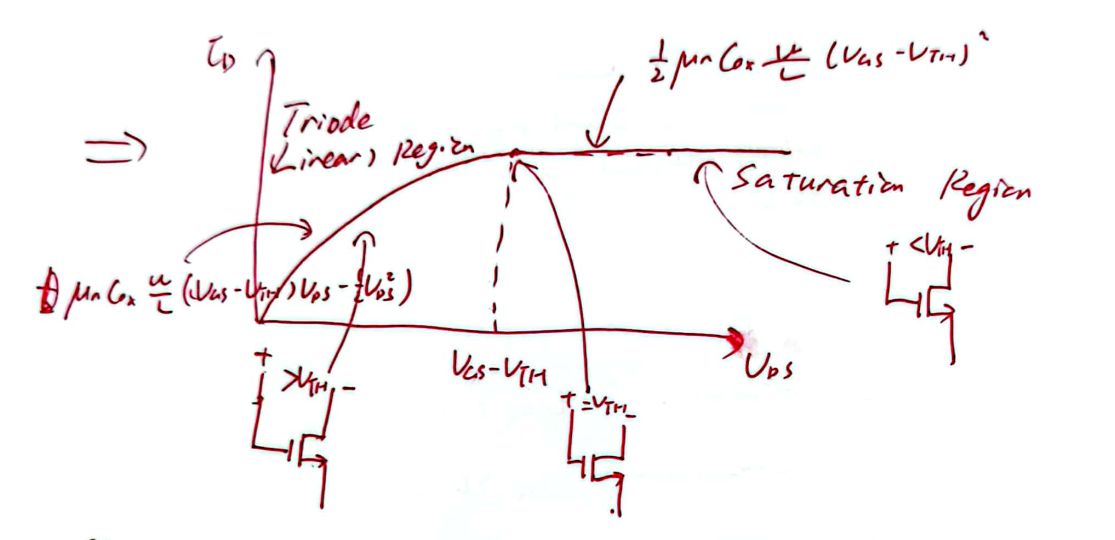
\includegraphics[scale=0.8]{5.jpg}
    \captionsetup{labelformat=empty}
    \caption{Relationship between $I_D$ and $V_{DS}$}
    \label{5}
\end{figure}

This also enlightens us that we only need to pay attention to the potential difference between the G and the D 
to judge the saturation region and the linear region. as the picture shows. 

\begin{figure}[htbp]
    \centering
    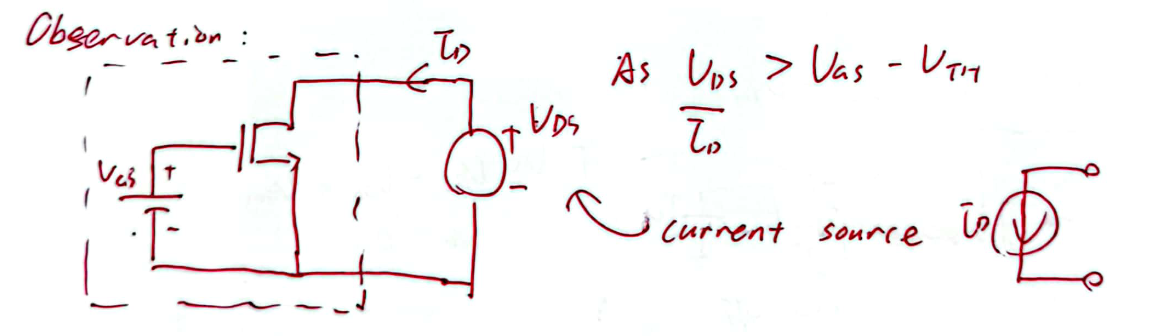
\includegraphics[scale=0.8]{6.jpg}
    \captionsetup{labelformat=empty}
    \caption{Current Source}
    \label{6}
\end{figure}

As $V_{DS}>V_{GS}-V_{TH}$, the $I_D$ is a constant. We can use this to make a current source. 

\subsection*{Relationship between $I_D$ and $V_{GS}$}

We can also derive the relationship between $I_D$ and $V_{GS}$. 

\begin{figure}[htbp]
    \centering
    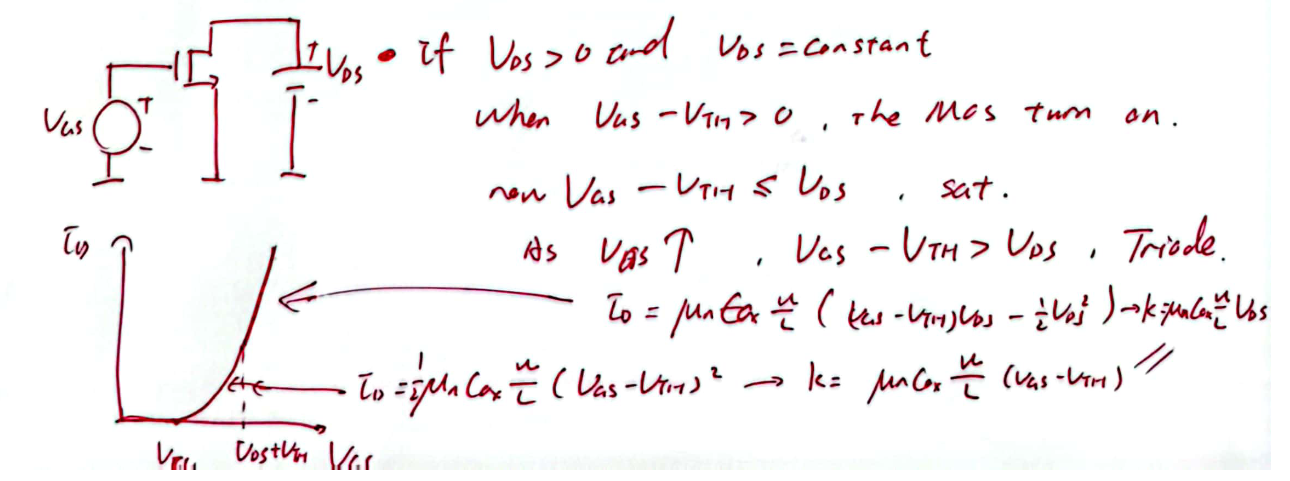
\includegraphics[scale=0.7]{7.jpg}
    \captionsetup{labelformat=empty}
    \caption{Relationship between $I_D$ and $V_{GS}$}
    \label{7}
\end{figure}

If $V_{DS}>0$ and $V_{DS}$ is a constant, when $V_{GS}>V_{TH}>0$, the MOS turns on. 
now $V_{GS}-V_{TH} \leq V_{DS}$, the MOS is in saturation zone. 

As $V_{GS}$ becomes larger, $V_{GS}-V_{TH}>V_{DS}$, the MOS is in triode zone. 

We can calculate for the curve, as I show in the picture. 

\section*{Simple Model in Saturation Zone}

\begin{figure}[htbp]
    \centering
    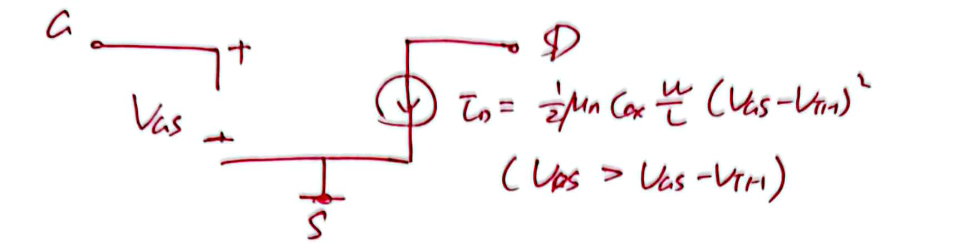
\includegraphics[scale=0.7]{8.jpg}
    \captionsetup{labelformat=empty}
    \caption{Use the Saturation to Design a Current Source}
    \label{8}
\end{figure}

\subsection*{Example}

$\mu C_{ox}=100\mu A/V^2$, $V_{TH}=0.5V$, $\frac{W}{L}=\frac{5\mu m}{0.5\mu m}$

Design a 1mA current source. 

$$I_D=\frac{1}{2}\mu_nC_{ox}\frac{W}{L}(V_{GS}-V_{TH})^2$$

we get $V_{GS}=1.91V$. 

Therefore, when $V_{DS}\geq 1.41V$, the MOS can be a current source with $I_D=1mA$. 

\section*{Link}

\href{https://www.bilibili.com/video/BV1FD4y1R7Ah?p=31&vd_source=1d0c07486a3bd3b0adb8ac548bf6453e}{Razavi Electronics Circuits 1: lectrue 31}
\end{document}